\documentclass[ngerman,aspectratio=169,10pt]{beamer}

\usetheme[progressbar=frametitle]{metropolis}
\usepackage{appendixnumberbeamer}

\graphicspath{{./graphics/}, {./../../figures/}}

\usepackage{booktabs}
\usepackage{xspace}
\usepackage{amsmath}
\usepackage{amssymb}
\usepackage{amsthm}
\usepackage{xfrac}
\usepackage{listings}
\lstset{
	basicstyle=\ttfamily,
	showstringspaces=false,
	tabsize=4,
	upquote=true,
}

\title{Verbesserungen}
% \subtitle{}
\date{03. Februar 2021}
\author{Levin Nemesch, Joshua Sangmeister}
\institute{Algorithm Engineering - Projekt}
\titlegraphic{
    \hfill
\includegraphics[height=1.5cm]{unilogo.pdf}\\
    \hspace*{8.3cm} \textsc{AG Theoretische Informatik}
}

\begin{document}

\maketitle

\begin{frame}{ILP-Formulierung}
	\textbf{Ansätze}:
    \begin{itemize}
        \item Alternative ILP-Formulierung
        \item Alternativer exakter Algorithmus: Reduzierung auf MaxClique
        \item ILP mit neuer Separationsheuristik
        \item ILP-Formulierung mit stärkeren Constraints
    \end{itemize}
\end{frame}

\begin{frame}{Alternative ILP-Formulierung}
	\textbf{TODO}
\end{frame}

\begin{frame}{Alternative ILP-Formulierung}
    \centering
    %\includegraphics[width=270px]{}\\ %folgt...
    $\longrightarrow$ deutlich langsamer
\end{frame}

\begin{frame}{Reduzierung auf MaxClique}
    \begin{itemize}
        \item Beobachtung: Optimale Lösung des Labeling-Problems bildet Clique maximaler Größe im dualen Konfliktgraphen, da alle Labels sich gegenseitig nicht überlappen dürfen
        \pause
        \item Aufbauen des dualen Konfliktgraphen, lösen mittels MCQD, Rücktransformation der Lösung
        \begin{itemize}
            \item MCQD: unter GNU General Public License veröffentlichter Algorithmus zur Lösung des MaxClique-Problems
       \end{itemize}
    \end{itemize}
    \pause
\end{frame}

\begin{frame}{Reduzierung auf MaxClique}
    \centering
    %\includegraphics[width=270px]{}\\ %folgt...
    $\longrightarrow$ deutlich langsamer
\end{frame}

\begin{frame}[fragile]{ILP mit Separationsheuristik}
    \begin{itemize}
        \item Zu Beginn nur Punkt-Constraints einfügen, keine Konflikt-Constraints
        \item Separationsheuristik:
        \begin{verbatim}
sort candidates descending by number of conflicts
foreach candidate with >=1 conflict:
    find max clique in this candidates conflicts
    add cut for all members of this clique
    remove conflicts of clique from graph
    break if "enough" cuts were generated
        \end{verbatim}
    \end{itemize}
    \pause
    $\longrightarrow$ deutlich langsamer
\end{frame}

\begin{frame}{ILP mit stärkeren Constraints}
    \begin{itemize}
        \item Beobachtung 1: einfach zu ermitteln, ob Punkt in einem anderen Label liegt
        \item Beobachtung 2: wenn Punkt in Label liegt, hat dieses Konflikte mit allen Kandidaten des Punktes
    \end{itemize}
    \pause
    $\longrightarrow$ Simple Verbesserung: Bei Generierung der Punkt-Constraints direkt alle Kandidaten mit einbeziehen, die den Punkt umschließen\\
    $\Longrightarrow$ stärkere Ungleichungen
\end{frame}

\begin{frame}{ILP mit stärkeren Constraints}
    \centering
    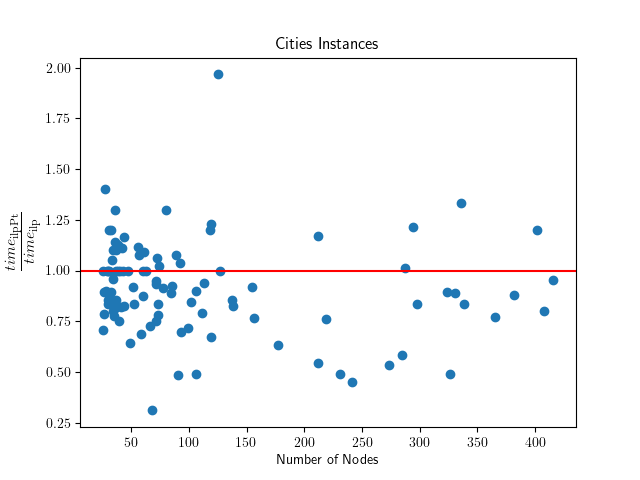
\includegraphics[width=270px]{time_ilppt_vs_ilp}\\
    Yay! Eine Verbesserung! (zumindest meistens...)
\end{frame}

\end{document}